In this part of our project, we have compared the performance of the five beamforming techniques using different antenna arrays,
in particular we have used as arrays:

\begin{enumerate}
    \item 2x2
    \item 4x4
    \item 8x8
    \item 16x16
\end{enumerate}

\subsection{Aim of the experiment}

The aim of this experiment is to evaluate the performance of different beamforming techniques using different antenna arrays. In 
particular, for each beamformer and for each antenna array, we have studied:

\begin{enumerate}
    \item The shape of the $QAM$ constellation revealed. 
    \item The shape of the array pattern function.
    \item The $BER$
\end{enumerate}

\subsection{Geometry and parameters}

In this simulation, we have considered two sources that we call $V1$ and $V2$: the signal we want to receive is the one from $V1$,
while $V2$ is producing an interfering signal.\\ 
Both the vehicles are not moving and they are transmitting 100 $4\-QAM$ symbols.\\
The geometry of the symulation can be seen in Figure \ref{fig:Scenario_still}.

\begin{figure}[ht]
    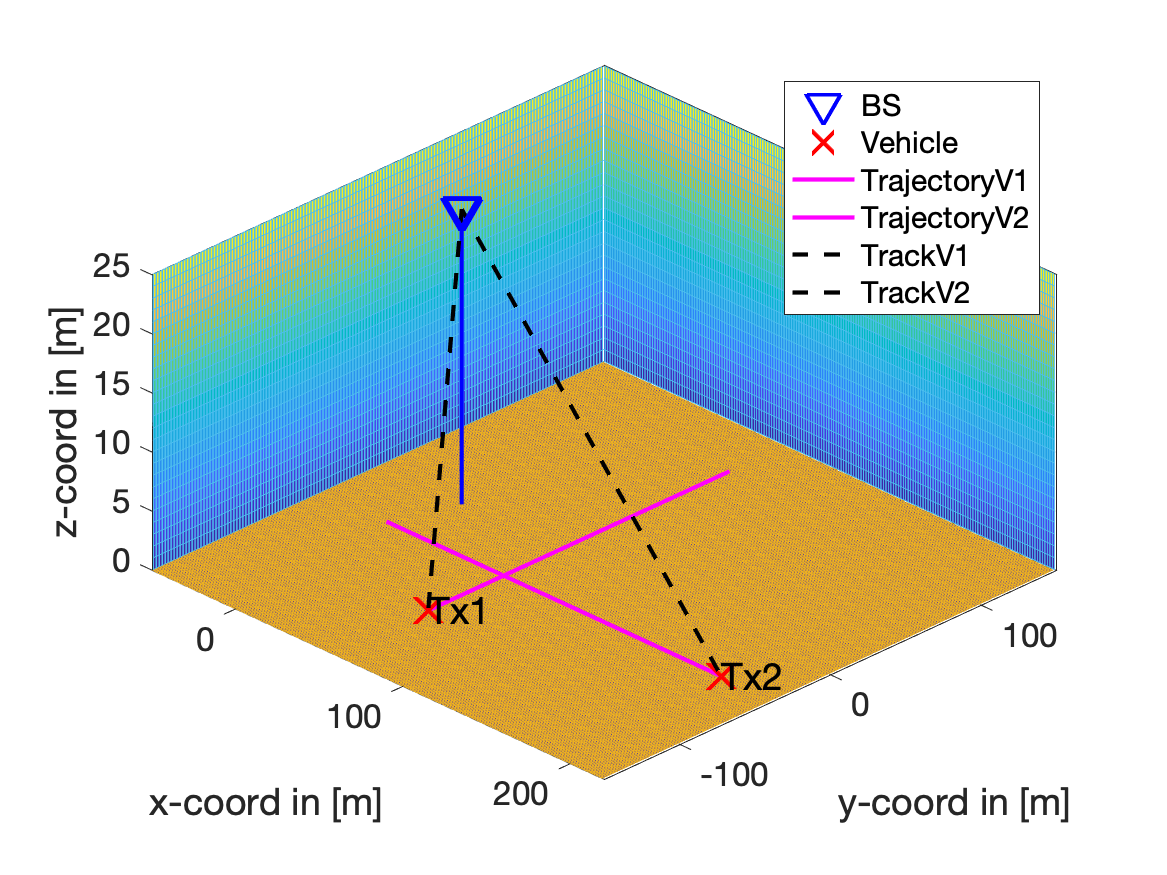
\includegraphics[width=\linewidth]{Quadriga1.png}
    \caption{Scenario of the simulation}
    \label{fig:Scenario_still}
\end{figure}

\subsection{Steps of the simulation}

The very first thing we do in our simulation is defining the geometry of our scenario, so positioning the vehicles and the base station.\\
Then, we prepare the signal to be transmitted, that is an OFDM signal modulating symbols from a 4\-QAM modulation.\\
The simulation proceeds with a loop on the four different antenna arrays. In each loop, the main steps we follow are:

\begin{enumerate}
    \item Definition of the current antenna array.
    \item Passage of the signal through the QuaDRiGa channel ($QuaDRiGa\_UD2D\_LOS$ scenario).
    \item Application of the five beamformers to the received signal. Here, we use the real $DoA$, and not the estimated one
            for a more consistent comparison of the results.
    \item Channel equalization using the gradient descent algorithm. Here, we use a one-tap equalizer since on each subcarrier 
            of the OFDM signal we can consider the channel as flat.
    \item OFDM demodulation.
    \item QAM demodulation.
    \item Computation of the BER.
\end{enumerate}

At the end of the loop, we show the results by making some plots and videos that are commented below in the following sections.

\subsection{Results: \textit{QAM} constellations}

In the Figure \ref{fig:Constellations} we can see 4 images, one per antenna array; in each one of them, we have
plotted the constellation revealed by using the five different beamformers. \\ 
As we can see, in general the higher the number of antenna we are using, the more precise is the $QAM$ constellation. This
is due to the fact that with more antenna the precision in the angular localization of the source is more precise; therefore, 
the beam that points towards it is narrower and the interfering signal is more attenuated (this can be seen even better by
looking at the antenna pattern functions).

\begin{figure}[ht]
    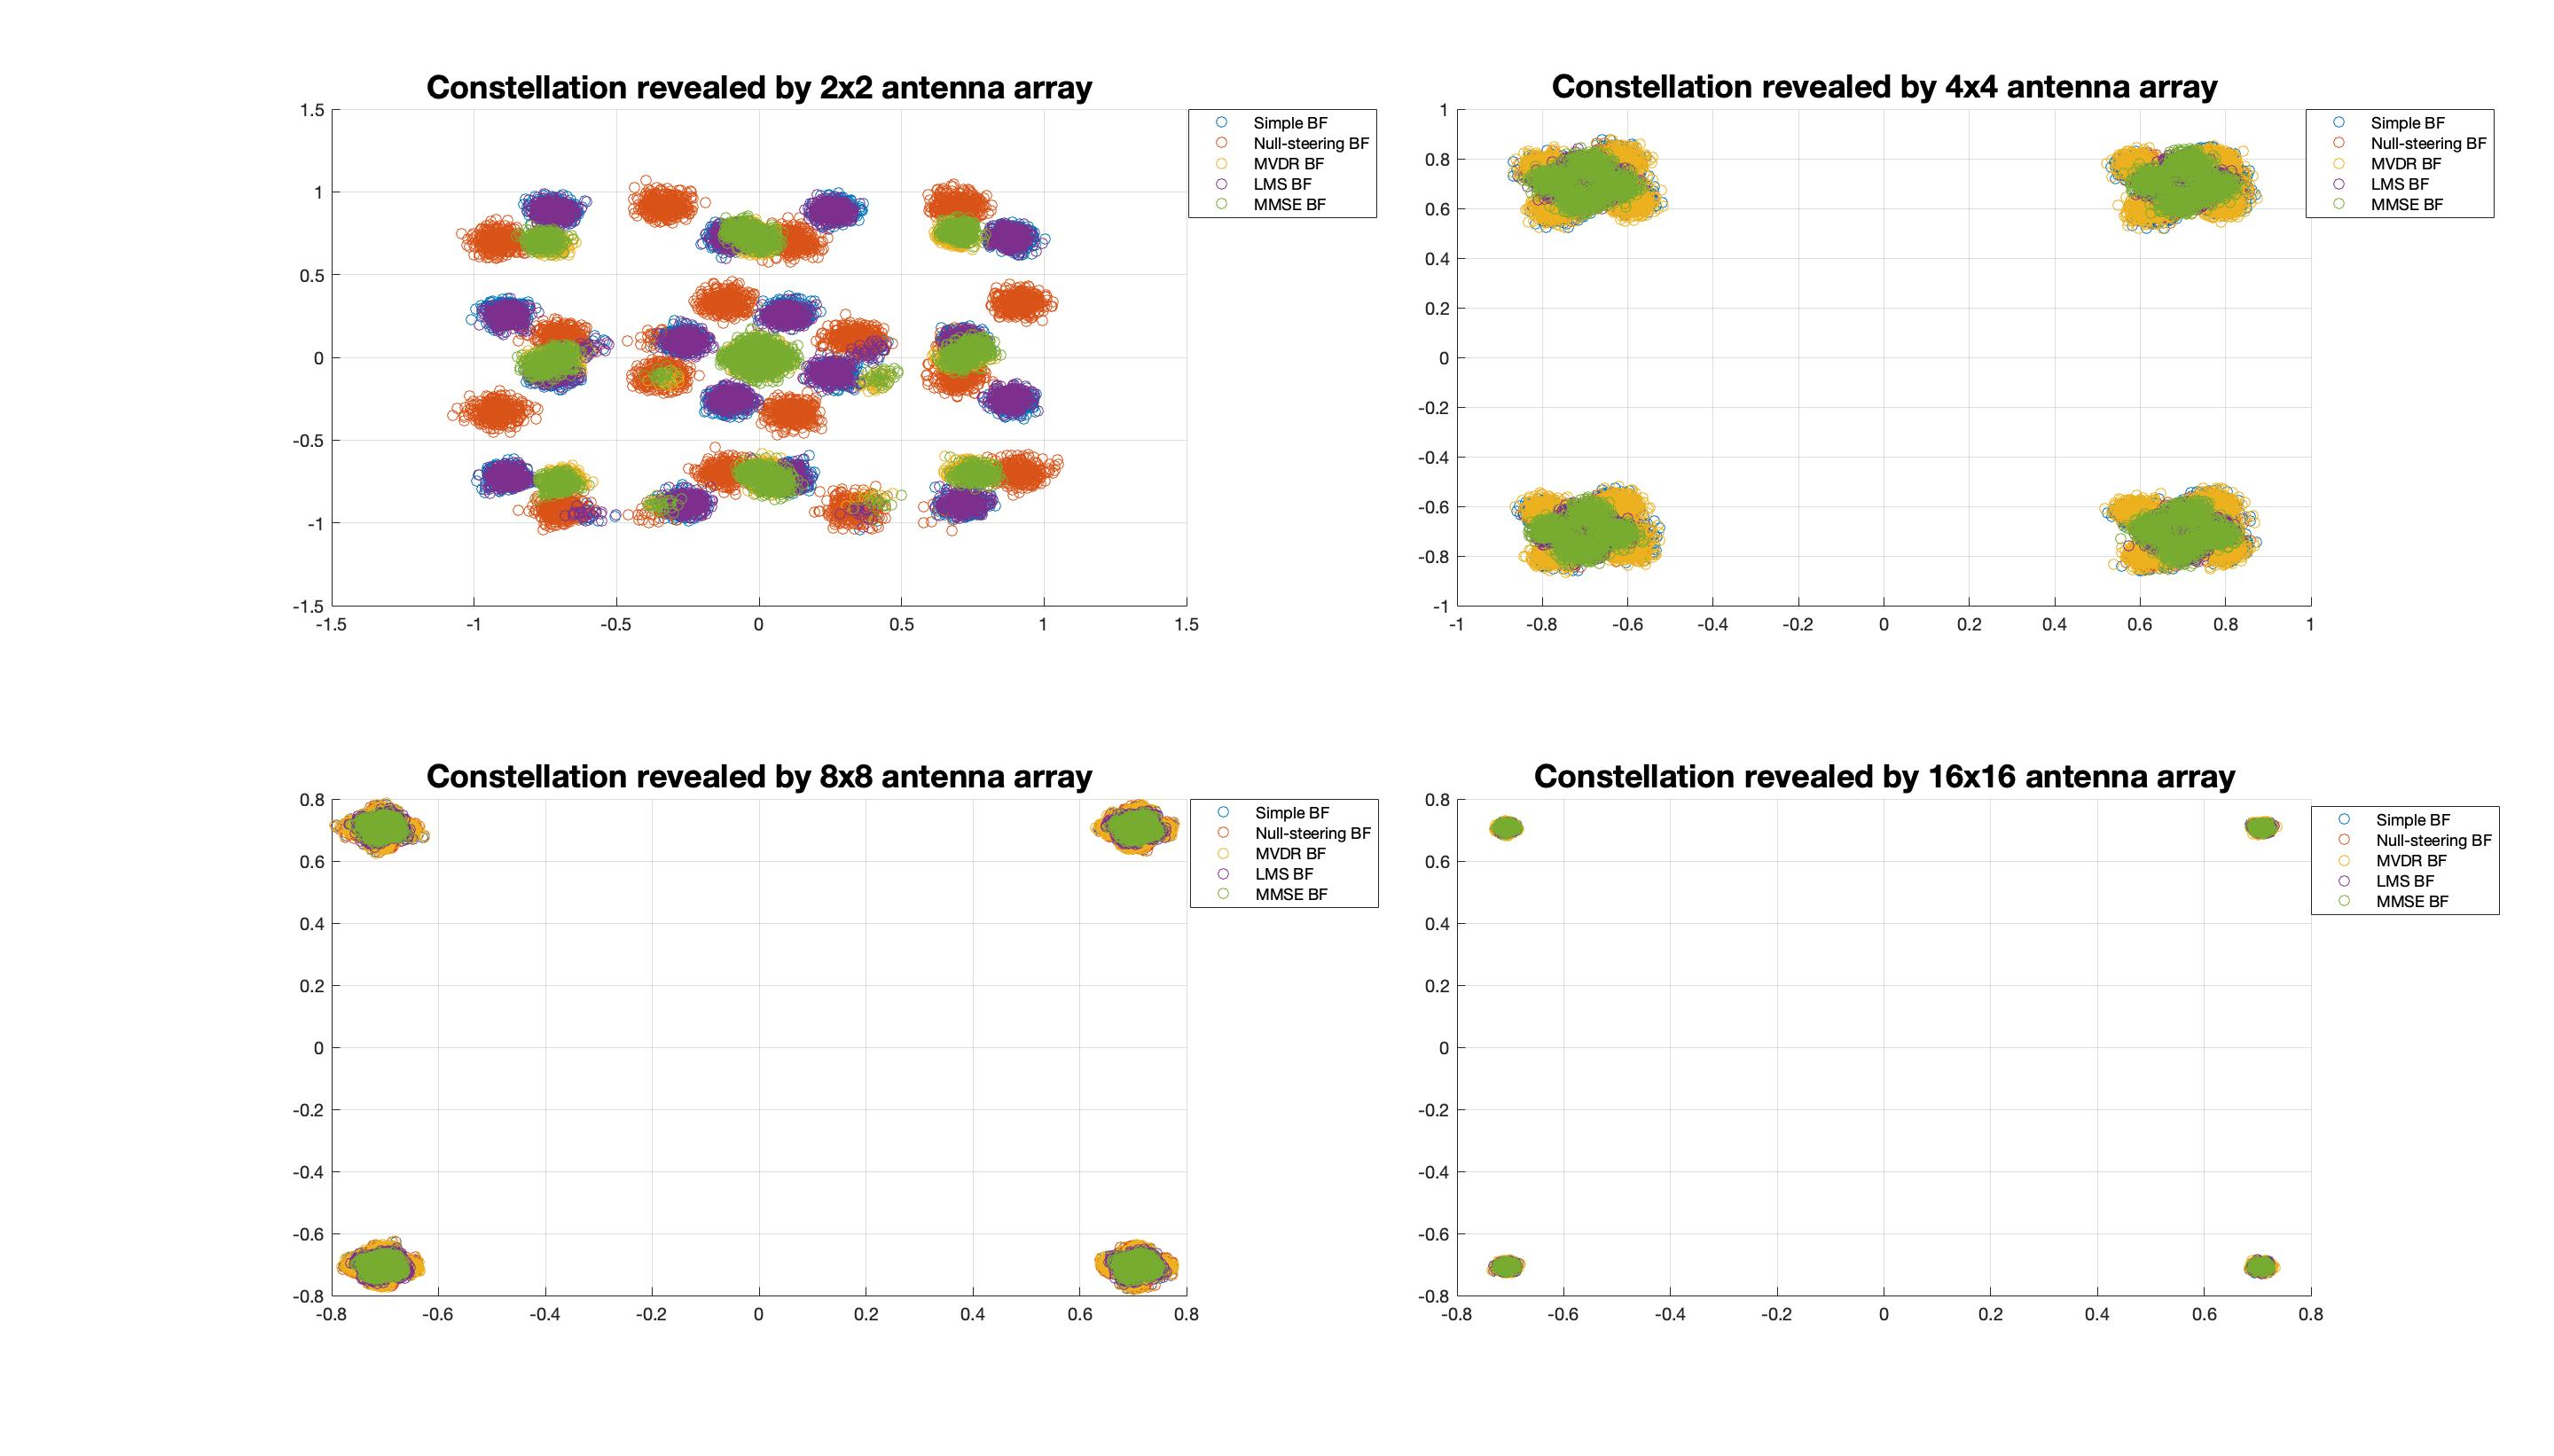
\includegraphics[width=\linewidth]{Constellations.jpg}
    \caption{4-QAM constellations}
    \label{fig:Constellations}
\end{figure}

\subsection{Results: antenna pattern functions}

The Figure \ref{fig:Array_pattern} shows for each of the four antenna arrays the array pattern function of the five
beamforming techniques we have implemented; the array pattern functions have been plotted on the zenith angles of the source.
We have also plotted a vertical line that represents the $DoA$ of the source.\\
The most interesting things to be noticed are two:

\begin{enumerate}
    \item The maximum of all the antenna array pattern functions is always localized in correspondence of the $DoA$ of the source.
            This is indeed the aim of beamforming.
    \item The higher the number of antennas, the narrower the beam that is pointing in the direction of the source. This is due 
            to the fact that with more antenna we have more spatial samples of the signal and therefore a better estimation of 
            its angular positions. 
\end{enumerate}

\begin{figure}[ht]
    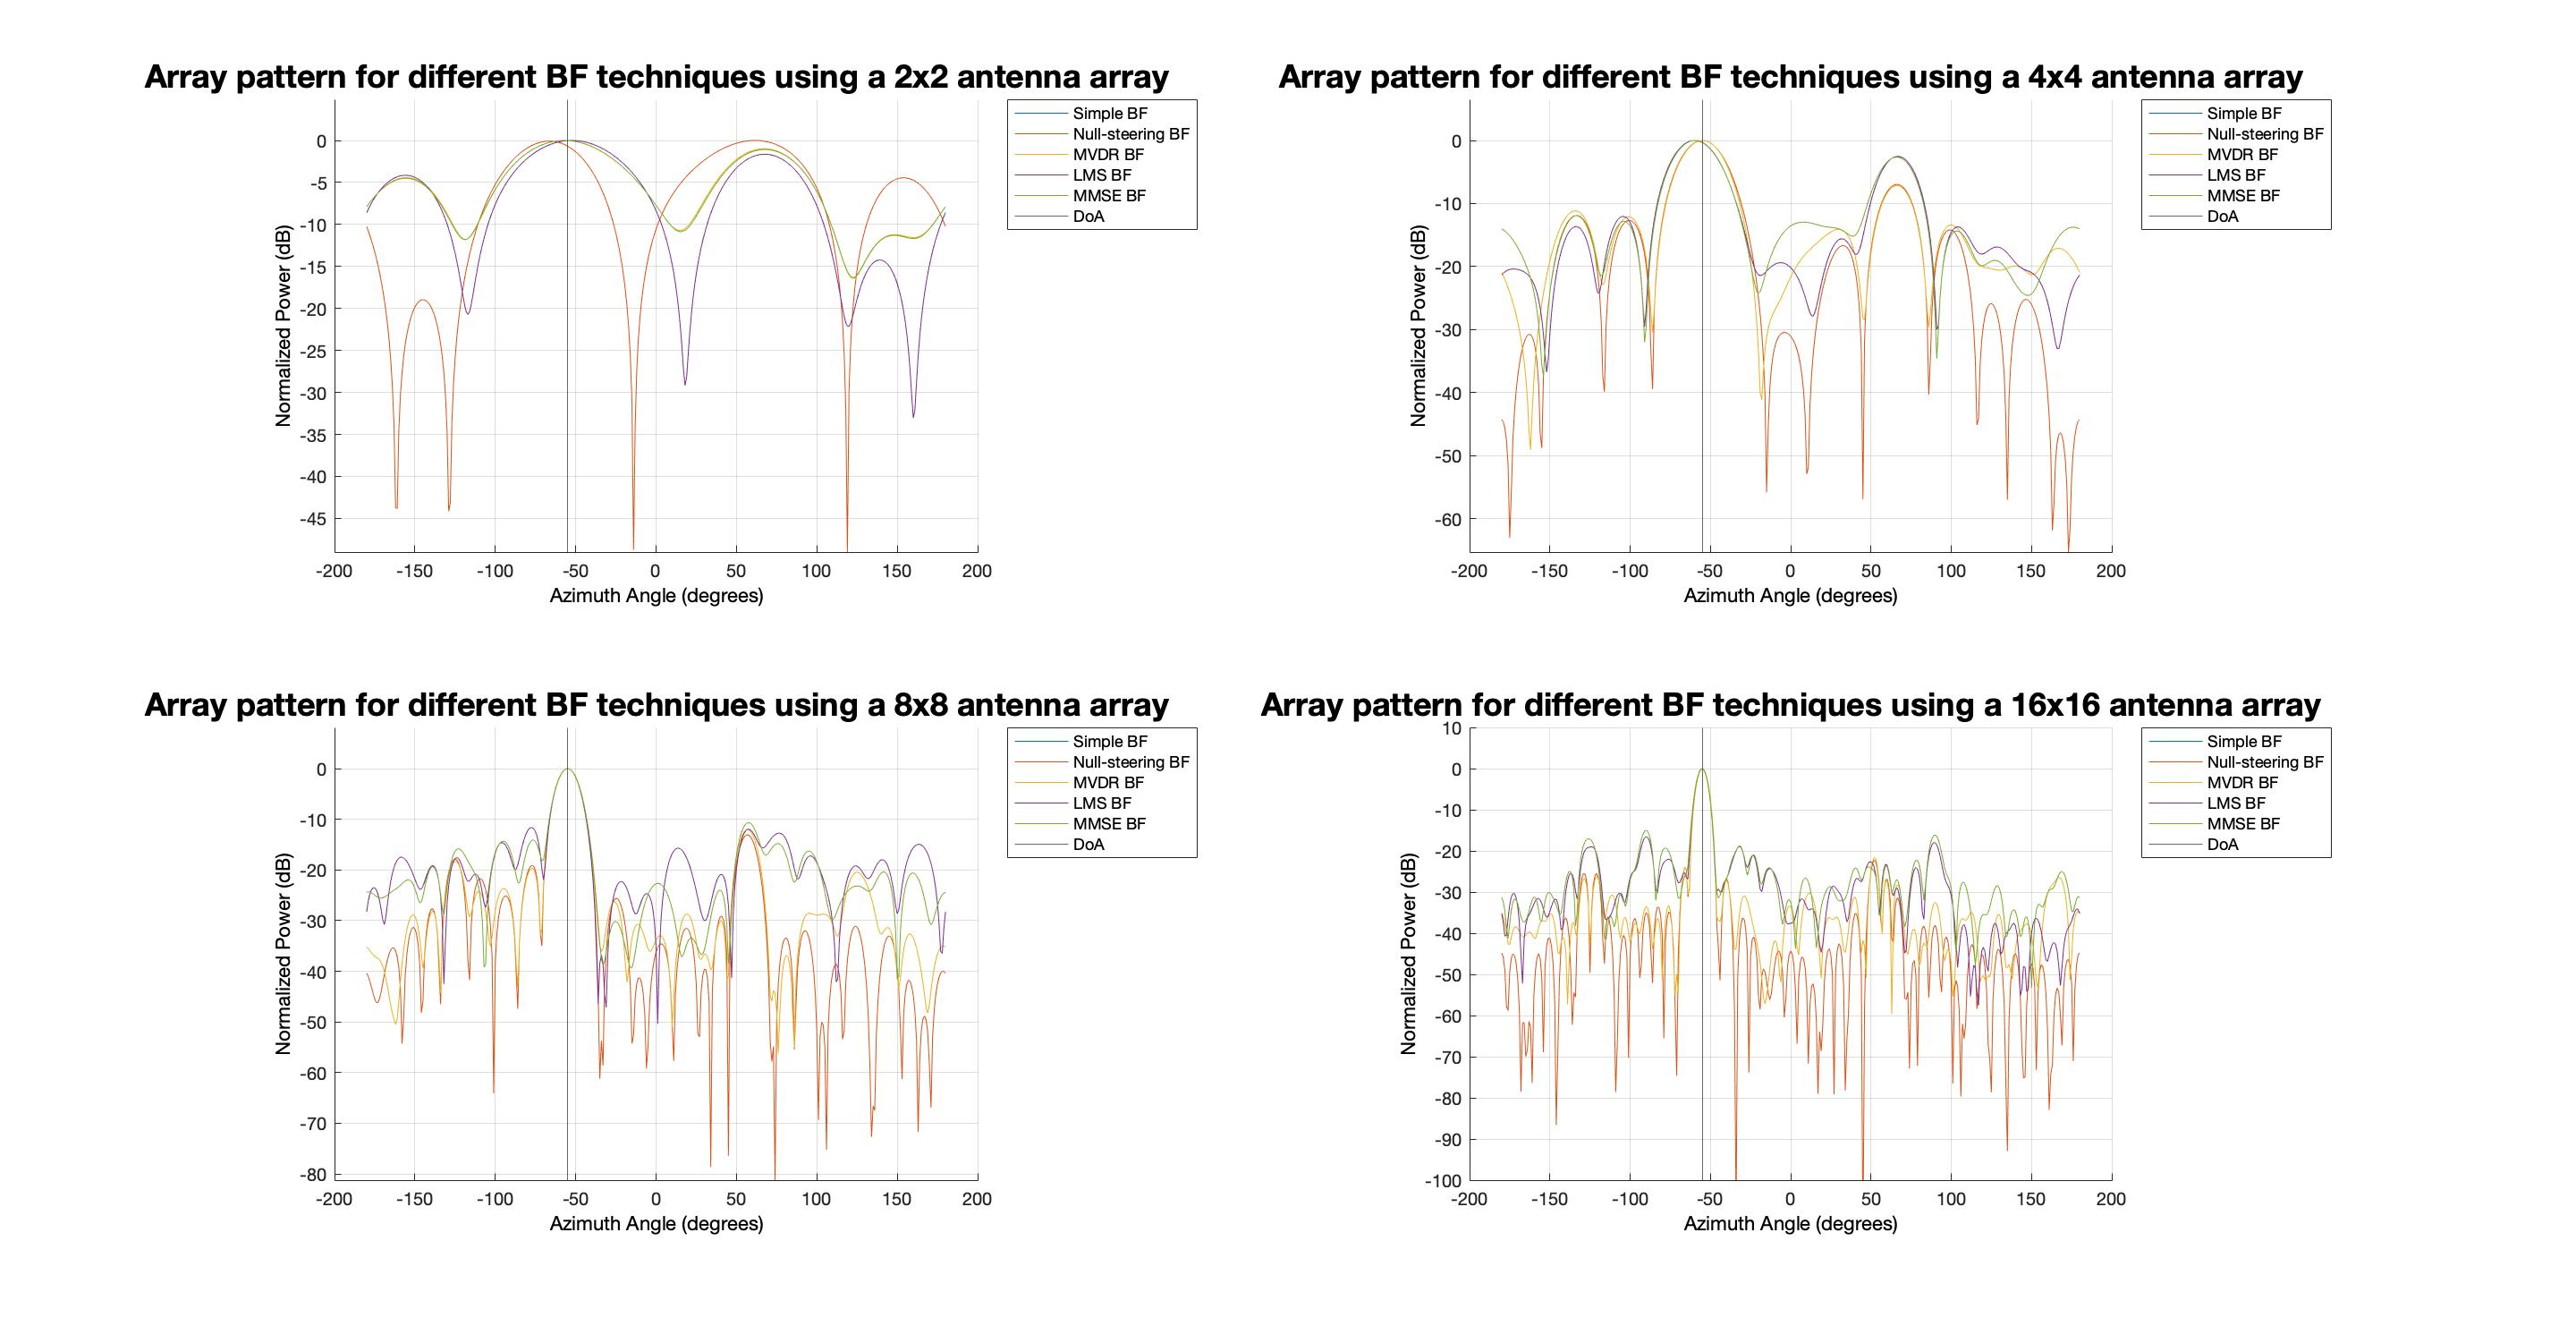
\includegraphics[width=\linewidth]{Array_pattern.jpg}
    \caption{Antenna pattern functions}
    \label{fig:Array_pattern}
\end{figure}

\subsection{Results: \textit{BER}}

Finally, the Figure \ref{fig:BER} shows how the $BER$ varies for the five beamformers as a function of the numberr of antennas.\\
As we can see, the $BER$ is different from zero only when we use the 2x2 antenna array. This means that four antennas may not
be sufficient for applying an effective beamforming technique. Actually, this also depends on the beamformer that we are using:
the more it's sophisticated, the less antennas we can use. But this also depends on the specific scenario. \\
What we can in general conclude is that the higher the number of antennas, the lower the $BER$; the actual number of antennas 
needed depends on the target $BER$ and on the model considered.

\begin{figure}[ht]
    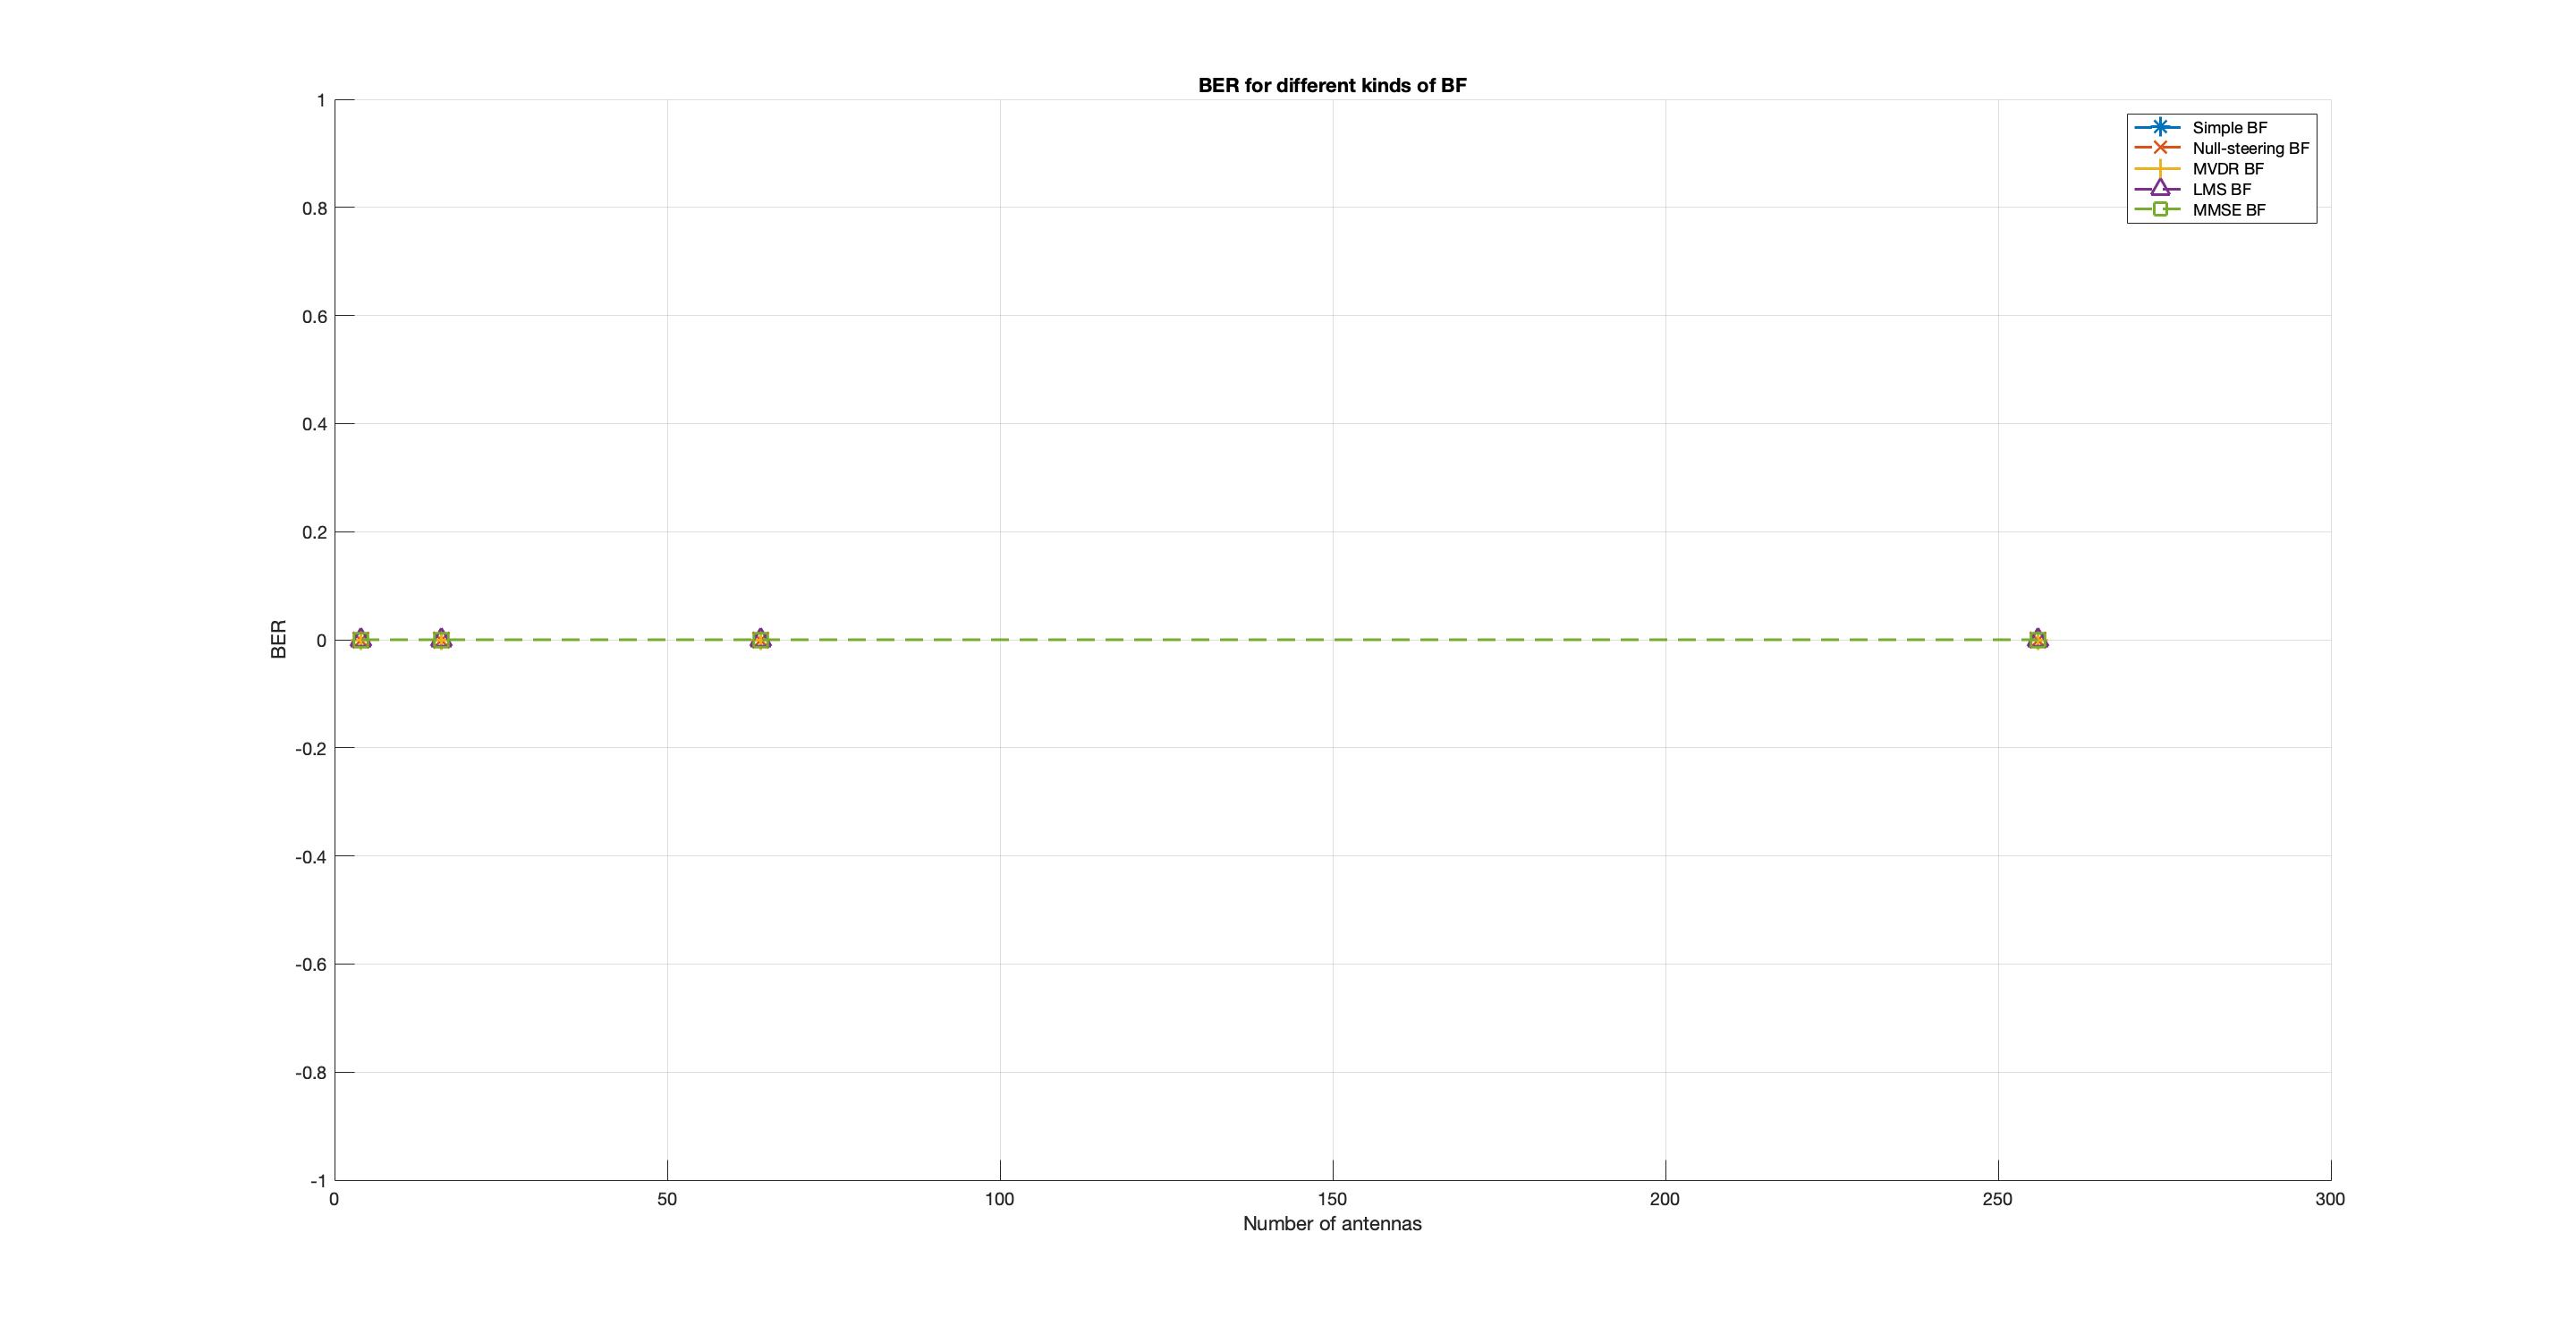
\includegraphics[width=\linewidth]{BER.jpg}
    \caption{BER}
    \label{fig:BER}
\end{figure}